\documentclass[../notes.tex]{subfiles}

\pagestyle{main}
\renewcommand{\chaptermark}[1]{\markboth{\chaptername\ \thechapter\ (#1)}{}}
\setcounter{chapter}{32}

\begin{document}




\chapter{The Nature and Propagation of Light}
\section{Light Wave Terminology and Basics}
\begin{itemize}
    \item \marginnote{8/10:}\textbf{Geometric optics}: The study of situations in which EM radiation interacts with objects (possibly with holes) such that $\lambda<<\text{size of obstacles, holes}$.
    \item \textbf{Physical optics}: The study of situations in which EM radiation interacts with objects (possibly with holes) such that $\lambda\approx\text{size of obstacles, holes}$.
    \item \textbf{Ray}: An imaginary line, perpendicular to the wave fronts, that indicates the direction of propagation.
    \item Any time a wave hits a medium, you get reflection and transmission.
    \item \textbf{Huygens principle}: All points on a wavefront act as point sources of spherical wavelets. After a time $\Delta t$, the new position of the wavefronts is the surface of tangency of the wavelets.
    \begin{figure}[h!]
        \centering
        \begin{tikzpicture}[
            every node/.append style={black}
        ]
            \footnotesize
            \draw [blx,thick] (0,0) -- ++(0,3);
            \draw [blx,semithick,densely dashed]
                (0,0.5) circle (4mm)
                (0,1.5) circle (4mm)
                (0,2.5) circle (4mm)
                (0,0.5) -- node[below,xshift=-2pt]{$r$} ++(135:0.4)
                (0,1.5) -- node[below,xshift=-2pt]{$r$} ++(135:0.4)
                (0,2.5) -- node[below,xshift=-2pt]{$r$} ++(135:0.4)
            ;
            \fill [blx]
                (0,0.5) circle (1.5pt)
                (0,1.5) circle (1.5pt)
                (0,2.5) circle (1.5pt)
            ;
    
            \draw [blx,thick,dash dot] (0.4,-0.5) -- ++(0,4);
            \node [align=center] at (1.5,3) {new\\wavefront}
                edge [out=-90,in=0,->,shorten >=1pt] (0.4,2)
            ;
        \end{tikzpicture}
        \caption{Huygens principle.}
        \label{fig:HuygensPrinciple}
    \end{figure}
    \begin{itemize}
        \item The radius $r$ of the wavelets, in terms of the time $\Delta t$ from their creation, is $r=c\Delta t$.
    \end{itemize}
    \item Light rays hitting a surface (see Figure \ref{fig:reflectingWaves}).
    \begin{figure}[h!]
        \centering
        \begin{subfigure}[b]{0.45\linewidth}
            \centering
            \begin{tikzpicture}
                \footnotesize
                \draw [semithick] (0,0) -- (5,0) coordinate (s) node[right]{Surface};
                \draw [dashed] (3.4,0) coordinate (P) -- ++(0,0.9) coordinate (Q);
                
                \draw [blx,thick] (0.2,0.8) -- ++(2.6,1.3);
                \draw [blx,thick] (0.45,0.3) -- ++(2.6,1.3);
                \draw [blx,thick] (1.1,0) coordinate (a) -- ++(2.2,1.1) coordinate (b);
    
                \draw [rex,thick,postaction={decorate},decoration={markings,mark=at position 0.45 with \arrowreversed{latex}}] (3.4,0) -- ++(-1.2,2.4) coordinate (R);
    
                \pic [draw,angle eccentricity=1.5,pic text={$\theta_1$},pic text options={yshift=-0.5pt}] {angle=s--a--b};
                \pic [draw,angle eccentricity=1.5,pic text={$\theta_1$},pic text options={xshift=0.5pt}] {angle=Q--P--R};
            \end{tikzpicture}
            \caption{Waves hit a surface.}
            \label{fig:reflectingWavesa}
        \end{subfigure}
        \begin{subfigure}[b]{0.45\linewidth}
            \centering
            \begin{tikzpicture}[
                every node/.append style={black}
            ]
                \footnotesize
                \draw [semithick] (0,0) coordinate (S) -- (5,0) coordinate (s) node[right]{Surface};
                
                \draw [blx,thick]
                    (1.1,0) coordinate (a) -- ++(4.4,2.2) coordinate (b)
                    (a) node[below left]{$A$} -- node[left]{$r$} ++(67.5:0.9) node[above right]{$B$}
                    (3.1,0) node[below right]{$D$} -- node[right]{$r$} ++(112.5:0.9) node[above left]{$C$}
                ;
                \draw [blx,thick,densely dashed]
                    (a) ++(9mm,0) arc[start angle=0,end angle=180,radius=9mm] ++(9mm,0)
                    ++(2,1) circle (9mm)
                    ++(2,1) circle (9mm)
                ;
                \fill [blx]
                    (a) circle (1.5pt)
                    ++(2,1) circle (1.5pt)
                    ++(2,1) circle (1.5pt)
                ;
                \draw [blx,thick,dash dot]
                    (3.1,0) -- ++(3,1.5)
                    (3.1,0) coordinate (A) -- ++(-2.4,1.2) coordinate (B)
                ;
    
                \pic [draw,angle eccentricity=1.5,pic text={$\theta_1$},pic text options={yshift=-0.5pt}] {angle=s--a--b};
                \pic [draw,angle eccentricity=1.5,pic text={$\theta_2$},pic text options={yshift=-0.5pt}] {angle=B--A--S};
            \end{tikzpicture}
            \caption{Invoking Huygens principle.}
            \label{fig:reflectingWavesb}
        \end{subfigure}\\[1em]
        \begin{subfigure}[b]{0.45\linewidth}
            \centering
            \begin{tikzpicture}
                \footnotesize
                \begin{scope}
                    \draw [blx,thick]
                        (0,0) coordinate (a) node[below left,black]{$A$}
                        -- node[left,black]{$c\Delta t$} ++(67.5:0.9) coordinate (b) node[above,black]{$B$}
                        -- (2,0) coordinate (c) node[below right,black]{$D$}
                        -- node{$|$} cycle
                    ;
                    \pic [draw,angle eccentricity=1.5,pic text={$\theta_2$},pic text options={yshift=-0.5pt}] {angle=b--c--a};
                    \pic [draw,angle radius=2mm] {right angle=a--b--c};
                \end{scope}
                \begin{scope}[xscale=-1,xshift=-6cm]
                    \draw [blx,thick]
                        (0,0) coordinate (A) node[below right,black]{$D$}
                        -- node[right,black]{$c\Delta t$} ++(67.5:0.9) coordinate (B) node[above,black]{$C$}
                        -- (2,0) coordinate (C) node[below left,black]{$A$}
                        -- node{$|$} cycle
                    ;
                    \pic [draw,angle eccentricity=1.5,pic text={$\theta_1$},pic text options={yshift=-0.5pt}] {angle=A--C--B};
                    \pic [draw,angle radius=2mm] {right angle=A--B--C};
                \end{scope}
            \end{tikzpicture}
            \caption{Proving identical triangles.}
            \label{fig:reflectingWavesc}
        \end{subfigure}
        \caption{Properties of reflecting waves.}
        \label{fig:reflectingWaves}
    \end{figure}
    \begin{itemize}
        \item Since the triangles containing the \textbf{angle of incidence} and the \textbf{angle of reflection} ($\triangle ACD$ and $\triangle ABD$, respectively) share $\overline{AD}$, $r$, and a right angle (see Figure \ref{fig:reflectingWavesc}), we have that they are identical.
        \item Thus, $\theta_1=\theta_2$.
        \item Since light rays have a constant phase offset (specifically, $\ang{90}$) from light waves, it follows that light rays also reflect off of surfaces with their original angle of incidence.
    \end{itemize}
    \item \textbf{Angle of incidence}: The angle with which wavefronts hit a surface, or the angle a light ray makes with a normal to a surface.
    \begin{itemize}
        \item The quantity $\theta_1$ in Figure \ref{fig:reflectingWaves}.
    \end{itemize}
    \item \textbf{Angle of reflection}: The angle with which the reflected wavefront intersects with a surface.
    \begin{itemize}
        \item The quantity $\theta_2$ in Figure \ref{fig:reflectingWavesb}.
    \end{itemize}
    \item \textbf{Law of reflection}: The principle that $\theta_1=\theta_2$.
\end{itemize}



\section{Reflection}
\begin{itemize}
    \item Corner reflector:
    \begin{figure}[h!]
        \centering
        \begin{tikzpicture}
            \footnotesize
            \draw [semithick] (0,2) coordinate (m1) node[above]{$M$} -- (0,0) coordinate (m2) -- (5,0) coordinate (m3) node[right]{$M$};
            \draw [very thin,dashed]
                (-0.8,0.9) -- ++(1.6,0) coordinate (n1)
                (1.8,-0.8) -- ++(0,1.6) coordinate (n2)
            ;
    
            \draw [
                rex,thick,postaction={decorate},
                decoration={
                    markings,
                    mark=at position 0.1  with \arrow{latex},
                    mark=at position 0.45 with \arrow{latex},
                    mark=at position 0.9  with \arrow{latex}
                }
            ]
                (2,1.9) coordinate (A)
                -- ++(-2,-1) coordinate (B)
                -- ++(1.8,-0.9) coordinate (C)
                -- ++(3,1.5) coordinate (D)
            ;
    
            \pic [draw,angle radius=2mm] {right angle=m1--m2--m3};
            \pic [draw,angle eccentricity=1.3,pic text={$\theta$}] {angle=n1--B--A};
            \pic [draw,angle eccentricity=1.3,pic text={$\theta$}] {angle=C--B--n1};
            \pic [draw,angle eccentricity=1.3,pic text={$\theta$}] {angle=B--C--m2};
            \pic [draw,angle eccentricity=1.3,pic text={$\ang{90}$\,-\,$\theta$},pic text options={xshift=-1mm,yshift=1mm}] {angle=n2--C--B};
            \pic [draw,angle eccentricity=1.3,pic text={$\ang{90}$\,-\,$\theta$},pic text options={xshift=1mm,yshift=1mm}] {angle=D--C--n2};
            \pic [draw,angle eccentricity=1.3,pic text={$\theta$}] {angle=m3--C--D};
        \end{tikzpicture}
        \caption{Corner reflector.}
        \label{fig:cornerReflector}
    \end{figure}
    \begin{itemize}
        \item The law of reflection implies that the ray entering at an angle $\theta$ will exit at the same angle, just displaced a bit.
    \end{itemize}
    \item If you don't want radar to detect planes:
    \begin{itemize}
        \item Eliminate right angles (they're corner reflectors).
        \item Make the surface something that absorbs radiation (hi tech ceramic).
    \end{itemize}
    \item Mirrors create images; tie to projective geometry.
    \begin{itemize}
        \item Seeing an object in the mirror is equivalent to seeing it as far behind the mirror as the thing is in front of the mirror.
        \item This is \textbf{ray tracing}!
    \end{itemize}
    \item \textbf{Virtual image}: An image that is created by light rays that don't really exist, i.e., projected light rays.
    \item Mirrors don't reverse left and right; they reverse front and back.
\end{itemize}



\section{Refraction}
\begin{itemize}
    \item Light waves and glass.
    \begin{itemize}
        \item Light waves enter glass, shake the atoms therein, and then those atoms emit their own light.
        \item However, the light emitted by the atoms goes in all directions.
        \item When you sum up all the secondary sources in a horrible integral, you end up with an effective wave propagating to the right, but at a speed less than the speed of light.
    \end{itemize}
    \item \textbf{Index of refraction}: The quotient of the speed of light in a vacuum and the speed of light in a particular medium. \emph{Denoted by} $\bm{n}$.
    \begin{equation*}
        n = \frac{c}{v}
    \end{equation*}
    \begin{itemize}
        \item Since light can never travel faster than the speed of light, $n\geq 1$.
        \item Some common $n$ values:
        \begin{itemize}
            \item $n_\text{water}\approx 1.33$.
            \item $n_\text{glass}\approx 1.5$.
            \item $n_\text{diamond}\approx 2.5$.
            \item $n_\text{air}\approx 1.003\approx 1$.
        \end{itemize}
    \end{itemize}
    \item In materials, $v$ changes and $f$ remains constant, so $\lambda$ changes.
    \begin{itemize}
        \item $c=f\lambda$ and $v=f\lambda'$ imply that
        \begin{equation*}
            \lambda' = \lambda\cdot\frac{v}{c} = \frac{\lambda}{n}
        \end{equation*}
    \end{itemize}
    \item In a surface, the wavefront gets bent.
    \begin{figure}[h!]
        \centering
        \begin{tikzpicture}[
            every node/.append style={black}
        ]
            \footnotesize
            \draw [semithick] (0,0) coordinate (S) -- (5,0) coordinate (s) node[right]{S};
            
            \draw [blx,thick]
                (1.1,0) coordinate (a) -- ++(4.4,2.2) coordinate (b)
            ;
            \draw [blx,thick,densely dashed]
                (a) ++(4.5mm,0) arc[start angle=0,end angle=-180,radius=4.5mm] ++(4.5mm,0)
                ++(2,1) circle (9mm)
                ++(2,1) circle (9mm)
            ;
            \fill [blx]
                (a) circle (1.5pt)
                ++(2,1) circle (1.5pt)
                ++(2,1) circle (1.5pt)
            ;
            \draw [blx,thick,dash dot]
                (3.1,0) -- ++(3,1.5)
                (3.1,0) coordinate (A) -- ++(-2.4,-0.6) coordinate (B)
            ;
    
            \pic [draw,angle eccentricity=1.5,pic text={$\theta_1$},pic text options={yshift=-0.5pt}] {angle=s--a--b};
            \pic [draw,angle radius=1.1cm,angle eccentricity=1.2,pic text={$\theta_2$},pic text options={yshift=0.2pt}] {angle=S--A--B};
        \end{tikzpicture}
        \caption{Properties of refracting waves.}
        \label{fig:refractingWaves}
    \end{figure}
    \begin{itemize}
        \item Similarly, the ray gets bent.
        \item When looking from air into a different surface, $\theta_2<\theta_1$.
        \item Explains why when you reach for something in water, it appears closer and in a different spot --- you're reaching for the virtual image!
    \end{itemize}
    \item \textbf{Angle of refraction}: The angle with which the refracted wavefront intersects with a surface.
    \begin{itemize}
        \item The quantity $\theta_2$ in Figure \ref{fig:refractingWaves}.
    \end{itemize}
    \item \textbf{Snell's law}: The formula $n_1\sin\theta_1=n_2\sin\theta_2$. \emph{Also known as} \textbf{law of refraction}.
    \item \textbf{Critical angle}: The angle of incidence such that light will be refracted at $\ang{90}$.
    \begin{itemize}
        \item If $\theta_\text{inc}>\theta_\text{crit}$, you only get reflection!
        \item From Snell's Law,
        \begin{equation*}
            \theta_\text{crit} = \sin^{-1}(n_2/n_1)
        \end{equation*}
    \end{itemize}
    \item \textbf{Total Internal Reflection}: Conditions such that all light is reflected and none is refracted. \emph{Also known as} \textbf{TIR}.
    \begin{itemize}
        \item Only a possibility when the light wave is moving to a medium with a lower index of refraction.
    \end{itemize}
    \item If you have a glass rod and you put light in at one end at an angle greater than the critical angle, it will be trapped and can only come out at the other end.
    \begin{itemize}
        \item Total internal reflection allows us to redirect light however we want.
        \item Light "flowing" through this construction is analogous to water flowing through a pipe.
        \item As long as the angle we bend the light pipe at isn't too sharp, it will stay trapped in the light pipe.
        \item In a well-designed light pipe, you will loose very little intensity.
        \item This is the principal behind fiber optics.
        \item You lose current in a wire due to resistance, but you don't lose much intensity in a light pipe.
    \end{itemize}
\end{itemize}



\section{Office Hours (Pandey)}
\begin{itemize}
    \item \marginnote{8/11:}Can you explain the upwards and downwards displacement currents in Figure \ref{fig:planarWavefront}?
    \begin{itemize}
        \item Not really.
    \end{itemize}
\end{itemize}



\section{Dispersion}
\begin{itemize}
    \item \marginnote{8/12:}The way that atoms shake in a material with light passing through it depends on the frequency of the light.
    \item Thus, $n=n(f)$.
    \begin{itemize}
        \item For example, $n_\text{blue}\neq n_\text{red}$.
    \end{itemize}
    \item In general, $n$ increases as $f$ increases (or $\lambda$ decreases).
    \begin{itemize}
        \item Thus, $n_\text{blue}>n_\text{red}$, for example.
    \end{itemize}
    \item Thus, if you have light made up of all kinds of different colors, every color will travel through the material at a different speed.
    \begin{figure}[h!]
        \centering
        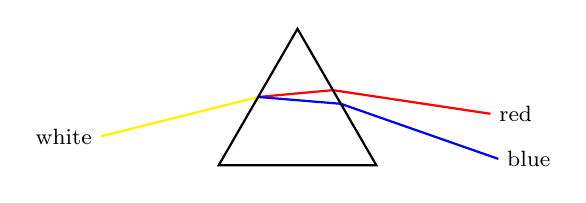
\begin{tikzpicture}[
            every node/.style={black}
        ]
            \footnotesize
            \draw [yellow,thick] (-120:1) -- ++(-2,-0.5) node[left]{white};
            \draw [red,thick] (-120:1) -- (-60:0.9) -- ++(2,-0.3) node[right]{red};
            \draw [blue,thick] (-120:1) -- (-60:1.1) -- ++(2,-0.7) node[right]{blue};
    
            \draw [thick] (0,0) -- (-60:2) -- (-120:2) -- cycle;
        \end{tikzpicture}
        \caption{A prism dispersing light.}
        \label{fig:prism}
    \end{figure}
    \begin{itemize}
        \item This is the principle behind a \textbf{prism}.
    \end{itemize}
    \item \textbf{Dispersion}: The dependence of the index of refraction on the frequency of light.
    \item When light passes through water droplets in the sky, it gets refracted by different amounts, depending on the color of the light. This is what creates a rainbow!
    \item \textbf{Fermat's Principle}: Light follows the path that takes the least time.
    \item Light traveling between $A$ and $B$ via a mirror.
    \begin{itemize}
        \item In this case, least time implies shortest distance.
        \item And indeed, the path with the shortest distance via the mirror is the one where $\theta_1=\theta_2$, as can be proven with optimization and calculus.
    \end{itemize}
    \item Light traveling between $A$ and $B$ via a change of medium.
    \begin{itemize}
        \item In this case, shortest distance \emph{does not} imply least time.
        \item If $n_1<n_2$, you can travel faster in $n_1$ then you can in $n_2$, so you want to minimize the time you spend in $n_2$ without going too far out of your way.
        \item It follows that the path with the least time will be the one given by Snell's law.
    \end{itemize}
    \item Why does light take the path of least time?
    \begin{itemize}
        \item Fermat says, "because it does."
        \item Quantum physics has a more bizarre reason for this.
    \end{itemize}
    \item How does light know which path to take?
    \begin{itemize}
        \item It doesn't --- it tries all paths and only one succeeds.
    \end{itemize}
\end{itemize}



\section{Polarization}
\begin{itemize}
    \item \marginnote{8/13:}Midterm on Tuesday.
    \begin{itemize}
        \item 80 minutes, more questions.
        \item HW 1-3.
        \item Chapter 15-16, 33-34.
    \end{itemize}
    \item \textbf{Polarized} (wave) \textbf{in the $\bm{xy}$-plane}: A wave where both the medium and displacement are entirely contained in the $xy$-plane. \emph{Also known as} \textbf{vertically polarized} (wave).
    \item If you shake a string up and down, you will create a polarized wave in the $xy$-plane.
    \item If you shake electrons up and down, you will create a vertically polarized EM wave, with $\vec{E}_\text{trans}$ entirely contained in the vertical plane.
    \begin{itemize}
        \item If you face said wave parallel to the propagation, you only see movement up and down.
    \end{itemize}
    \item A metal comb running vertically blocks vertically polarized microwaves since the microwaves lose energy creating currents in the metal.
    \begin{itemize}
        \item Works with microwaves since they're long, but wouldn't with visible light.
        \item However, a polaroid does work with the visible spectrum.
    \end{itemize}
    \item A polaroid filter is composed of long, stretched out organic molecules analogous to the teeth on the metal comb.
    \begin{itemize}
        \item If the \textbf{transmission axis} is vertical, all vertical waves get through.
        \item If it is horizontal, they all get blocked.
        \item If it is rotated at some angle $\phi$ from the vertical, decompose the radial vector into parallel and perpendicular components.
        \begin{itemize}
            \item The perpendicular component is totally blocked, and the parallel component is totally transmitted.
            \item It follows that $\vec{E}=\vec{E}_\parallel=\vec{E}_\text{polarized}\cos\phi$, so the wave amplitude of vertically polarized light decreases by $\cos\phi$.
        \end{itemize}
    \end{itemize}
    \item Since $I\propto A^2$, we get the following.
    \item \textbf{Law of Malus}: The following formula, where $I_2$ is the intensity of light that gets past the polaroid filter and $I_1$ is the initial intensity.
    \begin{equation*}
        I_2 = I_1\cos^2\phi
    \end{equation*}
    \item For unpolarized light, $I_\text{trans}=I_\text{unpol}\cos^2\phi$, but for light at every angle $\phi$.
    \begin{itemize}
        \item Thus, if we average $\cos^2\phi$ over all $\phi$, we get that
        \begin{equation*}
            I_\text{trans} = \frac{1}{2}I_\text{unpol}
        \end{equation*}
        \item Note that the above result is for a \textbf{perfect filter}. In reality, stacking filters causes some additional loss of intensity.
    \end{itemize}
    \item If you put a two filters on top of each other at perpendicular angles, it will entirely eliminate the intensity.
    \begin{itemize}
        \item At some angle $\phi$ in between, you'll have a variable loss of intensity.
    \end{itemize}
    \item If you put a third filter at an angle between two perpendicular filters, you'll regain some intensity.
\end{itemize}




\end{document}